\PassOptionsToPackage{unicode=true}{hyperref} % options for packages loaded elsewhere
\PassOptionsToPackage{hyphens}{url}
%
\documentclass[
]{book}
\usepackage{lmodern}
\usepackage{amssymb,amsmath}
\usepackage{ifxetex,ifluatex}
\ifnum 0\ifxetex 1\fi\ifluatex 1\fi=0 % if pdftex
  \usepackage[T1]{fontenc}
  \usepackage[utf8]{inputenc}
  \usepackage{textcomp} % provides euro and other symbols
\else % if luatex or xelatex
  \usepackage{unicode-math}
  \defaultfontfeatures{Scale=MatchLowercase}
  \defaultfontfeatures[\rmfamily]{Ligatures=TeX,Scale=1}
\fi
% use upquote if available, for straight quotes in verbatim environments
\IfFileExists{upquote.sty}{\usepackage{upquote}}{}
\IfFileExists{microtype.sty}{% use microtype if available
  \usepackage[]{microtype}
  \UseMicrotypeSet[protrusion]{basicmath} % disable protrusion for tt fonts
}{}
\makeatletter
\@ifundefined{KOMAClassName}{% if non-KOMA class
  \IfFileExists{parskip.sty}{%
    \usepackage{parskip}
  }{% else
    \setlength{\parindent}{0pt}
    \setlength{\parskip}{6pt plus 2pt minus 1pt}}
}{% if KOMA class
  \KOMAoptions{parskip=half}}
\makeatother
\usepackage{xcolor}
\IfFileExists{xurl.sty}{\usepackage{xurl}}{} % add URL line breaks if available
\IfFileExists{bookmark.sty}{\usepackage{bookmark}}{\usepackage{hyperref}}
\hypersetup{
  pdftitle={Una aproximación matemática a la fórmula de un indicador},
  pdfauthor={Valentina Londoño Ramirez},
  pdfborder={0 0 0},
  breaklinks=true}
\urlstyle{same}  % don't use monospace font for urls
\usepackage{longtable,booktabs}
% Allow footnotes in longtable head/foot
\IfFileExists{footnotehyper.sty}{\usepackage{footnotehyper}}{\usepackage{footnote}}
\makesavenoteenv{longtable}
\usepackage{graphicx,grffile}
\makeatletter
\def\maxwidth{\ifdim\Gin@nat@width>\linewidth\linewidth\else\Gin@nat@width\fi}
\def\maxheight{\ifdim\Gin@nat@height>\textheight\textheight\else\Gin@nat@height\fi}
\makeatother
% Scale images if necessary, so that they will not overflow the page
% margins by default, and it is still possible to overwrite the defaults
% using explicit options in \includegraphics[width, height, ...]{}
\setkeys{Gin}{width=\maxwidth,height=\maxheight,keepaspectratio}
\setlength{\emergencystretch}{3em}  % prevent overfull lines
\providecommand{\tightlist}{%
  \setlength{\itemsep}{0pt}\setlength{\parskip}{0pt}}
\setcounter{secnumdepth}{5}
% Redefines (sub)paragraphs to behave more like sections
\ifx\paragraph\undefined\else
  \let\oldparagraph\paragraph
  \renewcommand{\paragraph}[1]{\oldparagraph{#1}\mbox{}}
\fi
\ifx\subparagraph\undefined\else
  \let\oldsubparagraph\subparagraph
  \renewcommand{\subparagraph}[1]{\oldsubparagraph{#1}\mbox{}}
\fi

% set default figure placement to htbp
\makeatletter
\def\fps@figure{htbp}
\makeatother

\usepackage[]{natbib}
\bibliographystyle{apalike}

\title{Una aproximación matemática a la fórmula de un indicador}
\author{Valentina Londoño Ramirez}
\date{2021-03-13}

\begin{document}
\maketitle

{
\setcounter{tocdepth}{1}
\tableofcontents
}
\hypertarget{portada}{%
\chapter*{Portada}\label{portada}}
\addcontentsline{toc}{chapter}{Portada}

\begin{center}
\includegraphics[width=0.5\linewidth]{ProtectoR/portada} \end{center}

\hypertarget{intro}{%
\chapter{Indicadores}\label{intro}}

Los indicadores, es el plural del término ``indicador'' y precisamente, como dice su nombre lo dice, es un elemento que se utiliza para indicar o señalar algo. En el sentido más formal, un indicador es una herramienta cuantitativa o cualitativa que brinda una señal con una interpretación única y lógica. En efecto, debe comprenderse que los indicadores tienen un objetivo en concreto con la intención de poder monitorear, adaptar y controlar distintos procedimientos a seguir. De ahí, resulta necesario decir que un indicador debe representar la relación entre dos o más variables a fin de que sea más simple el análisis y la toma de decisiones respecto a la gestión de los resultados.

Existen diferentes maneras de clasificar los indicadores, dependiendo de su función y contexto en donde este actúa. A continuación describiremos sólo tres tipos de indicadores con el fin de que el lector pueda identificar su alcance frente a cualquier campo. Para empezar, mencionamos en qué consisten los \emph{indicadores de eficacia}. Estos tienen como propósito medir el grado de cumplimiento de una meta o un resultado propuesto. Asimismo, le sigue los \emph{indicadores de eficiencia} que miden el nivel de ejecución del proceso teniendo en cuenta la relación entre el logro del programa y los recursos utilizados para su cumplimiento mediante el tiempo, el esfuerzo o el costo. Por último, están los \emph{indicadores de calidad}, como su nombre lo dice, consiste en medir el nivel de calidad de un proceso o servicio mediante diferentes perspectivas como el nivel de satisfacción o la precisión en la ejecución del proceso.

Para poder entender mejor lo anterior, daremos algunos ejemplos a grandes rasgos desde la perspectiva de la universidad y cómo actúan los indicadores a partir de un objetivo establecido.

\begin{table}

\caption{\label{tab:unnamed-chunk-2}Ejemplos de indicadores}
\centering
\begin{tabular}[t]{l|l|l}
\hline
Dependencia & Objetivo & Indicadores\\
\hline
Bienestar universitario & Mantener la acreditación institucional y de alta calidad de sus programas académicos. & * Determinar el nivel de satisfacción en los usuarios de los servicios ofrecidos por Bienestar. <br> * El porcentaje  de estudiantes que califica con satisfacción alta o muy alta los servicios ofrecidos por bienestar académico.\\
\hline
Dirección académica & Contribuir a la internacionalización y bilingüismo como necesidad de la interacción con comunidades extranjeras. & * Medir el crecimiento de estudiantes extranjeros activos en la universidad.<br> * Costo que vale para la universidad dar un acompañamiento y seguimiento a un estudiante extranjero.<br> * Número de cursos de diferentes  idiomas no remotos ofertados por la universidad.\\
\hline
Investigación & Fomentar el desarrollo de investigación formativa e investigación científica en cada programa académico. & * Porcentaje de grupos de investigación activos en la universidad. <br> * Número de eventos, seminarios o espacios de difusión para compartir resultados y experiencias de un tema en común. <br> * Número de horas semanales dedicadas por cada estudiante al grupo de investigación.\\
\hline
Planeación institucional & Contribuir al desarrollo de políticas institucionales de buen gobierno que garanticen la estabilidad de cada programa académico. & * Determinar el nivel de participación entre cada ente que conforma la comunidad universitaria. <br> * Número de espacios asamblearios en cada programa académico de la universidad.\\
\hline
\end{tabular}
\end{table}

Como bien fue dicho, un indicador debe presentar la relación entre dos variables para ello es necesario definir un método de cálculo para el indicador. Por consiguiente, es preciso comprender la proporción, el porcentaje, la razón, la tasa de variación y el índice como métodos de cálculo más utilizados. Para ello, haremos un estudio detallado desde la estructura y el comportamiento matemático de cada uno de estos métodos.

\hypertarget{proporciuxf3n}{%
\chapter{Proporción}\label{proporciuxf3n}}

Matematicamente, la proporción es un cociente donde el numerador está incluido en el denominador cuyo objetivo es establecer la relación entre una parte con respecto al todo, en otras palabras es la relación que se establece entre un subconjunto \(n\) de un conjunto universo \(N\) y se define como
\[\begin{equation}
\text{Proporción de}\hspace{2mm}n=\frac{\text{Número de elementos de}\hspace{2mm}n}{\text{Total de elementos en el universo de}\hspace{2mm} N}
\end{equation}\]
donde \(n\) es un subconjunto de \(N\).Observe que el numerador siempre está incluido en el denorminador. Veamos el siguiente ejemplo.

\begin{longtable}[]{@{}l@{}}
\toprule
\begin{minipage}[b]{0.97\columnwidth}\raggedright
Ejemplo. \emph{Proporción de mujeres y hombres en una empresa}\strut
\end{minipage}\tabularnewline
\midrule
\endhead
\begin{minipage}[t]{0.97\columnwidth}\raggedright
En una empresa trabajan 27 mujeres y 18 hombres. Entonces podemos deducir que el total de trabajadores es \(27+18=45\) y por tanto la proporción de mujeres es \[\frac{\text{Número de mujeres}}{\text{Total de trabajadores}}=\frac{27}{45}=\frac{3}{5}\]. Similarmente, la proporción de hombres es \[\frac{\text{Número de hombres}}{\text{Total de trabajadores}}=\frac{18}{45}=\frac{2}{5}\]. En la empresa existen tres mujeres por cinco trabajadores y dos hombres por cada cinco trabajadores.\strut
\end{minipage}\tabularnewline
\bottomrule
\end{longtable}

Notemos que al ser el numerador una parte del denominador, el primero
nunca será más grande que el segundo. Esta es la razón por la que el resultado no puede ser mayor que la unidad y oscila siempre entre cero y uno.

\begin{table}

\caption{\label{tab:unnamed-chunk-3}Ejemplo de proporciones en la Universidad Nacional}
\centering
\begin{tabular}[t]{l|l|l}
\hline
Nombre del indicador & Método de cálculo & Procedimiento\\
\hline
Porporción de matriculados extranjeros de pregrado en la universidad en el período \$2020-I\$ & Número de  matriculados extranjeros de pregrado en la universidad en el periodo \$2020-I\$ /Total de estudiantes matriculados de pregrado en el periodo \$2020-I\$ & \$\{300\}/\{36.358\}=0,008\$\\
\hline
Proporción de matriculados de pregrado en el área de ciencias sociales y humanas de la universidad en el periodo \$2020-I\$. & Número total matriculados de pregrado en el área de ciencias sociales y humanas en el período \$2020-I\$/Total de estudiantes matriculados de pregrado en el período \$2020-I\$ & \$\{5.946\}/\{36.358\}=0,16\$\\
\hline
Proporción de aspirantes para pregrado por estrato socioeconómico 2 o menos de la universidad en el período \$2019-I\$. & Número total de aspirantes para pregrado por estrato socioeconómico 2 o menos en el período \$2019-I\$/Total de aspirantes para pregrado en el período \$2019-I\$ & \$\{48.639\}/\{82.854\}=0,58\$\\
\hline
\end{tabular}
\end{table}

Tomado de \citep{BibEntry244021Mar}

Las proporciones son muy utilizadas en los cálculos estadísticos, sin embargo por simplicidad se acostumbre multiplicar por 100 el resultado final. Cuando esto pasa llamaremos a la proporción como \protect\hyperlink{porcentaje}{\emph{porcentaje}}. Veamos más ejemplos de proporciones.

Como lo hace notar \citet{franco2016estadistica} en epidemiología, las proporciones permiten expresar la frecuencia de los eventos de salud, la enfermedad y las lesiones, en términos de su incidencia o prevalencia; es decir entre los casos nuevos o los casos existentes ocurridos. También permite mostrar en qué medida una población está expuesta a un
determinado factor de riesgo.

\begin{longtable}[]{@{}l@{}}
\toprule
\begin{minipage}[b]{0.97\columnwidth}\raggedright
Ejemplo. \emph{Proporción anual de muertes en una población}\strut
\end{minipage}\tabularnewline
\midrule
\endhead
\begin{minipage}[t]{0.97\columnwidth}\raggedright
Si en un año en una población de 450 habitantes se presentaron 10 muertes. Entonces \[\text{Proporción anual de muertes}=\frac{\text{Número de personas fallecidas en el año}}{\text{Población total}}=\frac{10}{450}=0,02\]\strut
\end{minipage}\tabularnewline
\bottomrule
\end{longtable}

En otros casos, las proporciones cuando se tratan de mediciones de peso, talla, espacio, volumen, etcétera; suelen llamarse fracciones. Por ejemplo, la masa de una parte de un cuerpo puede expresarse como una fracción de su masa total.

\hypertarget{razuxf3n}{%
\chapter{Razón}\label{razuxf3n}}

Una razón es una comparación multiplicativa de dos o más cantidades o medida.

\begin{quote}
La razón entre \(a\) y \(b\) cuando \(b\) es una cantidad distinta de cero, se escribe:
\(\frac{a}{b}\) o \(a:b\) y se lee \(a\) es a \(b\).
\end{quote}

Véase también \citep{huircan2013guia}.

Esta relación nos da cuántas veces una cantidad es igual a la otra cantidad, como 6 estudiantes por 1 profesor o 2 tazas de azúcar para 5 tazas de harina. Independientemente de la situación, las comparaciones de razones siempre se relacionan de forma multiplicativa. Por ejemplo, la razón de 6 estudiantes por 2 profesores es que hay 3 veces más estudiantes que profesores. También se puede describir esta relación de varias formas, tales como:

\begin{itemize}
\tightlist
\item
  3 estudiantes por cada profesor.
\item
  Un profesor por cada 3 estudiantes.
\item
  El número de profesores es \(\frac{1}{3}\) del número de estudiantes.
\end{itemize}

Independientemente de la forma en que se comunique esta relación, debe ser claro que hay 3 veces más estudiantes que profesores.

Cabe mencionar que, como lo afiman \citep{petit2020focus} la razón puede tener dos interpretaciones. La primera es por
unir o componer dos cantidades de una manera que ``conserva una relación multiplicativa'', es decir, un cierto número de una cantidad junto con un cierto número de otra cantidad crea un compuesto unidad \citep{beckmann2017mathematics}. Por ejemplo,

\includegraphics[width=0.3125in,height=\textheight]{https://static.vecteezy.com/system/resources/previews/001/209/957/non_2x/square-png.png} \includegraphics[width=0.3125in,height=\textheight]{https://static.vecteezy.com/system/resources/previews/001/209/957/non_2x/square-png.png} \includegraphics[width=0.3125in,height=\textheight]{https://static.vecteezy.com/system/resources/previews/001/209/957/non_2x/square-png.png} \includegraphics[width=0.29167in,height=\textheight]{https://www.nicepng.com/png/detail/926-9260681_cuadro-cuadrados-borde-monochrome.png}

\begin{enumerate}
\def\labelenumi{\arabic{enumi}.}
\tightlist
\item
  La relación de cuadros blancos a cuadros negros es \(\frac{1}{3}\) ó \(1:3\).
\end{enumerate}


\includegraphics[width=0.05\linewidth]{ProtectoR/estumate}

\includegraphics[width=0.05\linewidth]{ProtectoR/estumate}

\includegraphics[width=0.05\linewidth]{ProtectoR/estumate}

\includegraphics[width=0.05\linewidth]{ProtectoR/estumate}

\includegraphics[width=0.05\linewidth]{ProtectoR/estumate}

\includegraphics[width=0.05\linewidth]{ProtectoR/estumate}

\includegraphics[width=0.05\linewidth]{ProtectoR/estumate}

\includegraphics[width=0.05\linewidth]{ProtectoR/estuesta}

\includegraphics[width=0.05\linewidth]{ProtectoR/estuesta}

\includegraphics[width=0.05\linewidth]{ProtectoR/estuesta}

\begin{enumerate}
\def\labelenumi{\arabic{enumi}.}
\setcounter{enumi}{1}
\tightlist
\item
  La relación de estudiantes de matemáticas a estudiantes de estadística es \(\frac{7}{3}\) ó \(7:3\).
\end{enumerate}


\includegraphics[width=0.52083in,height=\textheight]{ProtectoR/arroz.png} 
\includegraphics[width=0.41667in,height=\textheight]{ProtectoR/harina.png}
\includegraphics[width=0.41667in,height=\textheight]{ProtectoR/harina.png}

Imágenes tomadas de \citet{BibEntry2021Marzo} y \citet{BibEntry2019Mar}.

\begin{enumerate}
\def\labelenumi{\arabic{enumi}.}
\setcounter{enumi}{2}
\tightlist
\item
  La relación entre libras de arroz a kilos de harina es \(\frac{1}{2}\) ó \(1:2\).
\end{enumerate}

Observemos que libras de arroz y kilos de lentejas son cantidades de medidas diferentes mientras que en el anterior, las cantidades solo eran estudiantes. Esto nos dice que las cantidades que componen una unidad compuesta pueden ser las mismas o diferentes.

La segunda interpretación consiste en comparar multiplicativamente dos cantidades. Por ejemplo, en una situación cotidiana en el que estamos comparando el precio de dos artículos, es conveniente notar cual es el artículo más costoso, de lo que lleva a decir: ``el artículo 1 es \(n\) veces más costoso que el artículo 2'', o también es válido decir: ``el artículo 2 vale \(\$5000\) más que el artículo 1. Sin embargo, la relación que ocurre es en términos multiplicativos contra aditivos. Por tanto, la primera expresión, la cual es dada en términos multiplicativos, es un ejemplo de razón como comparación multiplicativa.

Precisamos advertir que la razón no es una fracción en el sentido matemático, la confusión puede deberse al hecho de que una de las notaciones para la razón, \(\frac{a}{b}\) donde \(b\neq 0\), comparte la misma forma con una fracción. Ilustremos mejor mediante el siguiente ejemplo:
En el primer parcial, Ana acierta en \(3\) preguntas y desacierta en \(10\) preguntas. Después en el segundo parcial responde bien \(5\) y desacierta en \(7\) preguntas . ¿Cuál es la razón de las preguntas acertadas con las desaciertas en los dos parciales?

Número de preguntas acertadas:
\(\frac{6 \hspace{2mm} aciertos}{10 \hspace{2mm} desaciertos}+\frac{4\hspace{2mm} aciertos}{7\hspace{2mm} desaciertos}=\frac{10 \hspace{2mm} aciertos}{17 \hspace{2mm} desaciertos}\).

Con lo que \(10\) aciertos es a \(17\) desaciertos.

Pero Ana siempre llega \(\frac{3}{4}\) de hora tarde a las clases los martes y \(\frac{5}{8}\) de hora tarde para clases los jueves. ¿Cuántas horas en total llega Ana tarde a las clases los martes y jueves?

Número de horas que llegar tarde:
\(\frac{3}{4}hora+\frac{5}{8}hora=\frac{11}{8}hora\)

Para concluir, tenemos que el primer contexto es un ejemplo de una situación de razón, y el segundo contexto es un ejemplo de una situación de fracción. Notemos que el primer ejemplo involucra cuatro cantidades: \(6\) aciertos es a \(10\) desaciertos y \(4\) aciertos es a \(7\) desaciertos en el segundo parcial. En contraste, el segundo ejemplo involucra sólo dos cantidades: \(\frac{3}{4}\) de hora y \(\frac{5}{8}\) de hora.

Por otro lado, cuando nos referimos a \(10 km/h\) realmente estamos comparando dos cantidades distintas, y se traduce como \emph{por cada hora se recorre 10 kilómetros} o también la relación entre kilometros y segundos es
\[\begin{equation}
\frac{10}{1}, \hspace{5mm} 10:1
\end{equation}\]
lo que nos dice es una razón. Estos tipos de razones que involucran un periodo de tiempo los llamaremos \protect\hyperlink{tasas}{\emph{tasas}}.

\hypertarget{porcentaje}{%
\chapter{Porcentaje}\label{porcentaje}}

Un porcentaje es la forma de expresar un número como partes de cada cien. Como ya se dijo, Los porcentajes son proporciones multiplicado por \(100\). De manera más clara, podemos construir indicadores de porcentaje aplicando la operación

\[\begin{equation}
\text{Porcentaje de}\hspace{2mm}n=\frac{\text{Número de elementos de}\hspace{2mm}n}{\text{Total de elementos en el universo de}\hspace{2mm} N}\times 100.
\end{equation}\]

El porcentaje se representa con el símbolo \(\%\), donde el conjunto \(N\) representa el \(100\) por ciento, y cada una de las relaciones obtenidas al dividir entre el total (elementos de \(N\)) y multiplicarlo por \(100\) representa un tanto de cien, y es definido como tanto por ciento.

Algunos ejemplos son los siguientes

\begin{table}

\caption{\label{tab:unnamed-chunk-5}Ambiente Escolar}
\centering
\begin{tabular}[t]{l|l|l}
\hline
Nombre del indicador & Método de cálculo & Procedimiento\\
\hline
Porcentaje de estudiantes vinculados a actividades de extensión en la universidad en el periodo \$2019-II\$. & Número de estudiantes vinculados a actividades de extensión en la universidad en el periodo \$2019-II /\$ Total de estudiantes matriculados en el periodo \$2019-II × 100\$ & \$\{3.600\}/\{54.284\} × 100=11,61\$\%\\
\hline
Porcentaje de tesis meritorias por estudiantes graduados en la universidad en el periodo \$2020-I\$. & Número total de tesis meritorias por estudiantes graduados en el universidad en el periodo \$2020-I /\$ Total de estudiantes graduados en el período \$2020-I × 100\$ & \$\{195\}/\{4.926\} × 100=3,95\$\%\\
\hline
Porcentaje de funcionarias administrativas en la universidad en el periodo \$2020-I\$. & Número de administrativos mujeres en el período \$2020-I/\$ Total de administrativos en el periodo \$2020-I × 100\$ & \$\{1.460\}/\{2.850\} × 100=51,2\$\%\\
\hline
\end{tabular}
\end{table}

Tomado de \citep{BibEntry244021Mar}

Adicional a esto, es importante mencionar los procedimientos en el cálculo de porcentajes: Por aplicación directa o por proporciones, los cuales sirven como ruta para determinar otros hallazgos del indicador.

\begin{itemize}
\tightlist
\item
  Por aplicación directa, para el cálculo del \(t\%\) de una cantidad \(N\) y es hallado mediante la expresión :
\end{itemize}

\[\begin{equation}
\frac{t}{100}\times N.
\end{equation}\]

\begin{longtable}[]{@{}l@{}}
\toprule
\begin{minipage}[b]{0.97\columnwidth}\raggedright
Ejemplo. Descuento de un artículo\strut
\end{minipage}\tabularnewline
\midrule
\endhead
\begin{minipage}[t]{0.97\columnwidth}\raggedright
Un almacén tiene el \(30\%\) de descuento en artículos de cocina. Para calcular el precio final de una licuadora que vale \(\$80.000\) debemos \(\frac{30}{100}\times 80.000=24.000.\) Es decir, \(\$24.000\) equivale al \(30\%\) de la licuadora y como es un \(30\%\) menos, entonces \(\$80.000-\$24.000=\$56.000\) es el precio final.\strut
\end{minipage}\tabularnewline
\bottomrule
\end{longtable}

\begin{itemize}
\tightlist
\item
  Por proporciones, es utilizado cuando se plantea una proporción asignando el \(100\%\) al total y se calcula mediante la expresión:
\end{itemize}

\[\begin{equation}
\frac{t\%}{x}=\frac{100\%}{N}
\end{equation}\]

\begin{longtable}[]{@{}l@{}}
\toprule
\begin{minipage}[b]{0.97\columnwidth}\raggedright
Ejemplo\strut
\end{minipage}\tabularnewline
\midrule
\endhead
\begin{minipage}[t]{0.97\columnwidth}\raggedright
La cantidad de mujeres socias de una cadena de supermercados es \(1.455\) de \(9.700\), cifra que podemos obtener mediante \(\frac{t\%}{1.455}=\frac{100\%}{9.700}\) y haciendo el debido despeje resulta el \(15\%\). Tambien son equivalentes las expresiones: 1,5 de cada 10, 12 de cada 80, 15 de cada 100 ó 0,15 de 1.\strut
\end{minipage}\tabularnewline
\bottomrule
\end{longtable}

Hemos visto, un porcentaje expresa una \protect\hyperlink{proporciuxf3n}{proporción}, es decir, una parte de un total.

\hypertarget{tasas}{%
\chapter{Tasas}\label{tasas}}

Una tasa es una razón entre dos cantidades con unidades distintas y expresan la dinámica de un suceso en una población a lo largo del tiempo. Si la tasa o la cantidad frente a la cual algo está cambiando no está especificada, usualmente la tasa es por unidad de tiempo. Sin embargo, una tasa puede ser especificada por unidad de tiempo, por unidad de medida o masa o cualquier otra cantidad. Naturalmente para describir las unidades de una tasa, la palabra ``por'' se utiliza para poder separar las unidades de dos medidas utilizadas para calcular la tasa como por ejemplo, pesos por libra, metros por segundo, millas por hora, y días enfermo por año. De aquí es conveniente clasificar algunas tasas cuando \emph{el denominador es una variable temporal, un ``stock'' poblacional} ó \emph{una variable monetaria}.

\textbf{\emph{1. Cuando el denominador es un ``stock'' poblacional}}. Haciendo referencia a un ``stock'' poblacional como las poblaciones en un punto exacto de tiempo y tienen como fuentes los censos, padrones, estimaciones de población o encuestas. Para el cálculo, el numerador expresa el número de eventos ocurridos en una población durante un período. Como afirma \citet{moreno2000principales}, a diferencia de las \protect\hyperlink{proporcion}{proporciones}, el denominador no expresa el número de sujetos en observación sino el tiempo durante el cual tales sujetos estuvieron en riesgo de sufrir el evento. Así que, la tasa se calcula mediante la siguiente fórmula

\(\frac{\text{Número de eventos ocurridos en un población en el periodo t}}{\text{Sumatoria de los periodos donde los individuos de la población libres del evento estuvieron expuestos al riesgo en el periodo t}}\times 10^n\)

La unidad de medida empleada se conoce como \emph{tiempo-persona} de seguimiento. Por ejemplo, la observación de 100 individuos libres del evento durante un año corresponde a 100 años-persona de seguimiento; de manera similar, 10 sujetos observados durante diez años corresponden a 100 años-persona. Entonces, la población \(n\) en observación durante un año corresponde a \(n\) año-persona. Así que, esto explica el porque en los ejemplos clásicos sobre tasas en epidemiología (algunos se presentarán a continuación) que corresponden a estudios hechos durante un período de un año, la sumatoria de los períodos donde los individuos de la población libres del evento estuvieron expuestos al ``riesgo'' en el periodo de un año (el denominador de la tasa) coindice con la población en observación.

\begin{itemize}
\tightlist
\item
  \emph{Tasa de natalidad:} Es el número de nacimientos de una población por cada \(10^n\) habitantes en un año.
  \[\frac{\text{Número de nacimientos en un periodo de tiempo}}{\text{Población media en ese periodo}}\times 10^n\]
\end{itemize}

El uso de la constante \(10^n\), responde a la necesidad de comunicar el indicador de una manera comprensible y de fácil uso o recordación con el fin de permitir rápidamente su comparación con otras hechos.

\begin{longtable}[]{@{}l@{}}
\toprule
\begin{minipage}[b]{0.97\columnwidth}\raggedright
Ejemplo. \emph{Tasa de natalidad de una población}\strut
\end{minipage}\tabularnewline
\midrule
\endhead
\begin{minipage}[t]{0.97\columnwidth}\raggedright
En una población nacieron \(73.010\) niños a la fecha frente a una población de \(5'000.000\) habitantes. La tasa de natalidad a la fecha es \(\frac{73.010}{5'000.000}\times 1.000=14,6\).\strut
\end{minipage}\tabularnewline
\bottomrule
\end{longtable}

La tasa de natalidad será de \(0,0146\). No obstante, al usar el factor de \(1.000\) la cifra se presenta como ``\(14,6\) nacimientos por cada \(1.000\) habitantes'' lo cual es evidentemente más claro.

\begin{itemize}
\item
  \emph{Tasa de mortalidad:} Es el número de fallecimientos con respecto a la población total por cada \(10^n\) habitantes en un año.
  \[\frac{\text{Número de difunciones en un periodo de tiempo}}{\text{Población media en ese período}}\times 10^n\]
\item
  \emph{Tasa de desempleados:} Mide el nivel de desocupación en relación con la población activa por cada \(10^n\) habitantes en un año.
  \[\frac{\text{Número de desempleados en un período de tiempo}}{\text{Población media en ese periodo}}\times 10^n\]
\end{itemize}

No siempre el ``stock'' poblacional representa la poblacion media de una región. Tambien puede ser una población con alguna caracteristica en cuestión, como lo veremos a continuación:

\begin{itemize}
\tightlist
\item
  \emph{Tasa de prevalencia:} Es una medida que dice cuantas personas sufren una enfermedad en una momento específico.
\end{itemize}

\[\begin{equation}
\frac{\text{Número de personas con la enfermedad en un periodo de tiempo}}{\text{Número de personas en la población expuesta al riesgo
en el momento}}\times 10^{n}
\end{equation}\]

\begin{itemize}
\tightlist
\item
  \emph{Tasa de letalidad:} Indica qué proporción de los diagnosticados con una enfermedad mueren por esa causa y su fórmula de cálculo es la siguiente:
\end{itemize}

\[\begin{equation}
\frac{\text{Número de muertes por una enfermedad en un perÍodo de tiempo}}{\text{Población dignosticada de la enfermedad en ese periodo}}\times 10^n
\end{equation}\]

\begin{longtable}[]{@{}l@{}}
\toprule
\begin{minipage}[b]{0.97\columnwidth}\raggedright
Ejemplo. \emph{Letalidad del cancer de páncreas}\strut
\end{minipage}\tabularnewline
\midrule
\endhead
\begin{minipage}[t]{0.97\columnwidth}\raggedright
En una población murieron \(266\) personas por cáncer de páncreas en el 2016 frente a un total de \(278\) personas diagnosticadas con cáncer de páncreas en ese mismo año. Se calcula que la tasa de letalidad sería \(\frac{266}{278}\times 100=95,7\%\).\strut
\end{minipage}\tabularnewline
\bottomrule
\end{longtable}

\textbf{\emph{2. Cuando el denominador es una variable temporal}}. Mide la frecuencia con la que, en un período de tiempo, aparece un suceso en una población. El cálculo de tasas se realiza dividiendo el total de eventos ocurridos en un periodo dado en una población entre el tiempo de observación en el que ocurrieron dichos eventos. Las tasas se expresan multiplicando el resultado obtenido por una potencia de \(10\), que puede variar entre \(10\) y \(100.000\).

\[\begin{equation}
\frac{\text{Número de eventos sucedidos}}{\text{Periodo en que fueron observados}}\times 10^{n}
\end{equation}\]

En efecto, magnitudes vectoriales como la velocidad que describe el cambio de posición con respecto al tiempo y la aceleración, el cambio de velocidad por unidad de tiempo son ejemplos de tasas muy comunes según esta clasificación. En otras áreas, también encontramos la tasa de flujo volumétrico, el cual relaciona el volumen de un líquido que pasa a través de un superfície dado por unidad temporal o la tasa de bits, en computación, que relaciona el número de bits enviados o procesados por un computador por unidad temporal.

\textbf{\emph{3. Cuando el denominador es una variable monetaria }}

\begin{itemize}
\tightlist
\item
  \emph{Tasa de cambio:} La tasa de cambio muestra la relación que existe entre dos monedas. Dicha tasa es un indicador que expresa cuántas unidades de una divisa se necesitan para obtener una unidad de la otra. En el caso de Colombia, tenemos la siguiente relación o también véase \citet{BibEntry2019Jun}.
\end{itemize}

\[\begin{equation}
\frac{\text{Cantidad o peso de la moneda local}}{\text{Una unidad de la moneda extrajera}}\times 10^{n}
\end{equation}\]

\begin{longtable}[]{@{}l@{}}
\toprule
\begin{minipage}[b]{0.97\columnwidth}\raggedright
Ejemplo. \emph{Tasa de cambio entre el euro y el dolar}\strut
\end{minipage}\tabularnewline
\midrule
\endhead
\begin{minipage}[t]{0.97\columnwidth}\raggedright
Si la tasa de cambio entre el euro y el dólar estadounidense fuera de 2,54. Esto implica a que el euro equivale a \(2,54\) dólares, es decir, \(\frac{2,54 \hspace{2mm} \text{dólares}}{1 \hspace{2mm}\text{euro}}= 2,54\).\strut
\end{minipage}\tabularnewline
\bottomrule
\end{longtable}

\begin{itemize}
\tightlist
\item
  \emph{Tasa Impositiva:} Se aplica para el pago de impuestos de una empresa.
\end{itemize}

\[\begin{equation}
\frac{\text{Impuestos pagados por la empresa en un periodo }}{\text{Ingresos obtenidos en el mismo periodo }}\times 10^{n}
\end{equation}\]

\hypertarget{tasavariaciuxf3n}{%
\section{Tasa de Variación}\label{tasavariaciuxf3n}}

Representa la razón de dos observaciones de una misma variable pero en dos diferentes puntos del tiempo (pasado y presente), por lo que expresa un cambio porcentual en el tiempo. La observación más reciente se coloca en el numerador mientras que la menos reciente se coloca en el denominador. Es decir para \(t,k\) números enteros, la tasa de variación se expresa como,

\[\begin{equation}
\frac{\text{(Variable en el periodo}\hspace{2mm} t)-(\text{Variable en el periodo} \hspace{2mm} t-k)}{\text{Variable en el periodo} \hspace{2mm} t-k} \hspace{8mm} \text{(1)}
\end{equation}\]

donde el numerador indica el cambio de la variable en relación a dichos períodos. En otras palabras, al ser una razón, se está comparando el cambio de la variable en dos períodos con la variable en el período menos reciente. Es equivalente de \((1)\) expresarlo

\[\begin{equation}
\frac{\text{Variable en el periodo}\hspace{2mm} t}{\text{Variable en el periodo} \hspace{2mm} t-k}-1
\end{equation}\]

finalmente se multiplica por \(10^{n}\) para expresar la tasa como una potencia de \(10\).

\[\begin{equation}
\left[\frac{\text{Variable en el periodo}\hspace{2mm} t}{\text{Variable en el periodo} \hspace{2mm} t-k}-1 \right] \times 10^{n}.
\end{equation}\]

Ahora es conveniente mencionar algunos ejemplos en donde se calcula la tasa de variación dado un indicador.

\begin{table}

\caption{\label{tab:unnamed-chunk-6}Tasas de variaciones de la Universidad Nacional}
\centering
\begin{tabular}[t]{l|l|l}
\hline
Nombre del indicador & Método de cálculo & Procedimiento\\
\hline
Tasa de variación del total de libros publicados en la universidad con o sin sello editorial entre los años \$2019-2020\$. & [(Total del libros publicados en el año \$2020 /\$ Total de libros publicados en el año \$2019\$)\$-1\$]\$×100\$ & [\$\{410\}/\{400\}-1\$]\$×100=2,5\$\%\\
\hline
Tasa de variación del total de docentes en la universidad entre los semestres \$2008-II\$ y \$2020-I\$. & [(Total de docentes  en el semestre \$2020-I /\$ Total de docentes en el semestre \$2008-II\$)\$-1\$]\$×100\$ & [\$\{3.113\}/\{2.940\}-1\$]\$×100=5,8\$\%\\
\hline
Tasa de variación del total de estudiantes matriculados en la universidad entre los semestres \$2009-II\$ y \$2020-I\$. & [(Total de estudiantes matriculados en el semestre \$2020-I /\$ Total de estudiantes matriculados en el semestre \$2009-II\$)\$-1\$]\$×100\$ & [\$\{54.284\}/\{45.200\}-1\$]\$×100=20\$\%\\
\hline
\end{tabular}
\end{table}

En la economía, encontramos otros ejemplos de tasa de variación.

\begin{itemize}
\tightlist
\item
  \textbf{\emph{Tasa de inflación:}} Muestra la variación porcentual de los precios de un determinado territorio, durante un período determinado y con esto, podemos saber como se han comportado los precios en un lugar determinado. El cálculo de esta tasa se determina en términos del \emph{Índice de Precios al Consumidor} (IPC) el cual es el encargado de recoger el cambio de los precios, mes a mes para evaluar el coste de la vida mediante artículos como alimentos, casa, transporte, cuidado de la salud, entretenimiento, ropa y otros gastos.
\end{itemize}

\[\begin{equation}
\left[\frac{\text{IPC actual}}{\text{IPC anterior}}-1\right]\times 10^{n}
\end{equation}\]

\begin{itemize}
\tightlist
\item
  \textbf{\emph{Tasa de crecimiento económico:}} Es la variación porcentual del PIB (Producto Interno Bruto) real en un período de tiempo determinado en el que pemite calcular cual ha sido el aumento de la cantidad de bienes y servicios que produce una economía \citep{de2009producto}.
\end{itemize}

\[\begin{equation}
\left[\frac{\text{PBI actual}}{\text{PBI anterior}}-1\right]\times 10^{n}
\end{equation}\]

\hypertarget{diferencia-entre-proporciuxf3n-y-tasa}{%
\chapter{Diferencia entre proporción y tasa}\label{diferencia-entre-proporciuxf3n-y-tasa}}

Según \citep{colimon1990fundamentos}, el concepto de tasa es similar al de una \protect\hyperlink{proporciuxf3n}{proporción}, como bien se dijo, con la diferencia de que las \protect\hyperlink{tasas}{tasas} llevan incorporado el concepto de tiempo haciendo referencia a la unidad de medida empleada tiempo-persona. Para comprender mejor como actua dicha diferencia, consideremos la proporción de incidencia vs.~la tasa de incidencia de una determinada población.

Antes de empezar, tengamos en cuenta que incidencia se refiere a los nuevos casos de una enfermedad en una determinada población, en un lugar dado y en un período específico. Con lo anterior, la \emph{proporción de incidencia} relaciona el numero de casos nuevos (numerador) con el total de individuos (denominador).

\begin{longtable}[]{@{}l@{}}
\toprule
\begin{minipage}[b]{0.97\columnwidth}\raggedright
Ejemplo. \emph{Proporción de incidencia de covid-19 en una población}.\strut
\end{minipage}\tabularnewline
\midrule
\endhead
\begin{minipage}[t]{0.97\columnwidth}\raggedright
Una población de 10.000 habitantes, registró 1.800 nuevos casos del Covid-19 en tres meses. Proporción de incidencia \(\times 1.000=\frac{1.800}{10.000}\times 1.000=180\) por mil.\strut
\end{minipage}\tabularnewline
\bottomrule
\end{longtable}

Ahora, cuando hablamos de \emph{tasa de incidencia} estamos midiendo la velocidad de presentación de una enfermedad durante un período. Notemos que una tasa consta de un numerador, que al igual que en la proporción, es el número de casos nuevos del evento, y de un denominador que es el número de unidades de tiempo-persona durante el cual pudo presentarse el evento.

\begin{longtable}[]{@{}l@{}}
\toprule
\begin{minipage}[b]{0.97\columnwidth}\raggedright
Ejemplo. \emph{Tasa de incidencia de covid en una población}\strut
\end{minipage}\tabularnewline
\midrule
\endhead
\begin{minipage}[t]{0.97\columnwidth}\raggedright
Una población de 10.000 habitantes, en un periodo de 3 meses registró 1.800 nuevos casos del Covid-19 en el mes de diciembre y con un total de 13.450 meses-persona de seguimiento. Tasa de incidencia \(\times 1.000=\frac{1.800}{4.850}\times 1.000=133,8\) por mil meses-persona.\strut
\end{minipage}\tabularnewline
\begin{minipage}[t]{0.97\columnwidth}\raggedright
Indica que por cada 1.000 meses-persona de seguimiento durante 3 meses, se presentaron aproximadamente 134 nuevos casos de covid-19.\strut
\end{minipage}\tabularnewline
\bottomrule
\end{longtable}

Tras haber leído el ejemplo anterior, es conveniente preguntarnos como se calculó el valor de 13.450 meses-persona y con que variables se relaciona. A manera de ilustración, consideraremos la siguiente tabla con el fin de tratar de explicar las tasas de incidencia dentro de un período de seguimiento de 3 meses.

\begin{table}

\caption{\label{tab:covid}Tasa de incidencia del Covid-19}
\centering
\begin{tabular}[t]{l|l|l|l|l}
\hline
Variables & Mes 1 & Mes 2 & Mes 3 & Total en los tres meses \\
\hline
*1). Período mensual* &  &  &  & \\
\hline
*2). Casos nuevos de Covid-19* & 200 & 600 & 1 & 1.8\\
\hline
*3). Nuevas entradas a la cohorte* & 100 & 500 & 1.1 & 1.7\\
\hline
|*4). Pérdidas en el seguimiento* \$=+3)-2)-4)\$ & 100 & 300 & 800 & 1.2\\
\hline
*5). Movimiento en el período* & -200 & -900 & -700 & 1.3\\
\hline
*6). Persona al principio del período* & 10 & 9.8 & 8.9 & 10\\
\hline
*7). Personas al final del período* \$=6)+5)\$ & 9.8 & 8.9 & 8.2 & 8.7\\
\hline
*8). Tiempo-persona en meses-persona*  \$=7) / 2)\$ & 4.9 & 4.45 & 4.1 & 13.45\\
\hline
*9). Tasa por 1.000* \$=2) / 8)×1000\$ & 40,8 & 134,8 & 243,9 & 133,8\\
\hline
\end{tabular}
\end{table}

\begin{quote}
\emph{2). Casos nuevos de Covid-19}: Constituye al numerador de la tasa en cada período y en el período total se suman los nuevos casos de Covid-19 de cada mes.
\end{quote}

\begin{quote}
\emph{3). Nuevas entradas a la cohorte}\footnote{\emph{cohorte}, es un tipo de investigación observacional y analítica en la que se hace una comparación de la frecuencia de aparición de un evento entre dos grupos, uno de los cuales está expuesto a un factor que no está presente en el otro grupo. En un cohorte dinámico, se presenta la entrada y salida de nuevos sujetos de estudio durante la fase de seguimiento, por lo que el número de miembros puede variar a través del tiempo.}: Consta de las nuevas entradas a la
cohorte hasta la fecha de cierre. Para el período total se suman las entradas de cadauno de los períodos anuales.
\end{quote}

\begin{quote}
\emph{4). Pérdidas en el seguimiento}: Son los retiros que se presentan por abandono debido a causas diferentes al evento de estudio (falta de cooperación, migración, muertes, etc.). Para el período total se suman las pérdidas de los tres meses.
\end{quote}

\begin{quote}
\emph{5). Movimiento en el período}: Es el balance final de entradas y salidas de
la cohorte. Este balance es positivo si hay más entradas que salidas y es negativo en el caso contrario. En la columna total, se suman los balances de los tres meses.
\end{quote}

\begin{quote}
\emph{6). Persona al principio del período}: Son las personas que pasan del
período anterior. Al principio del primer período mensual éstos son los
mismos individuos de la cohorte inicial (10.000). Los individuos que hay al principio del segundo período, son los que comenzaron la cohorte del período inicial más el balance positivo o negativo de este mismo período (Movimiento en el período), por ejemplo, para el mes 2: \(10.000-200=9.800\) y para el mes 3: \(9.800-900=8.900\). Los que inician el período total son los mismos que inician la cohorte en el primer mes (10.000).
\end{quote}

\begin{quote}
\emph{7). Personas al final del período}: Se calcula sumando las filas 6) y 5). Tenga en cuenta si las personas al final del período se incrementan si el balance de la fila (5) es positivo y disminuyen si por el contrario el balance es negativo.
\end{quote}

\begin{quote}
\emph{8). Tiempo-persona en meses-persona}: En este ejemplo, la unidad se contará en meses-persona. Para el período total, sería la suma de todos los meses-persona de los diferentes períodos, en nuestro caso, sería: 13.450 meses-persona. Esta fila constituye el denominador de la tasa en cada período.
\end{quote}

\begin{quote}
\emph{9). Tasa por k}: En nuestro caso \(k=1.000\). Constituye al valor de la tasa de incidencia en los diferentes periodos por cada 1.000 habitantes, siendo en el período total, el valor de la tasa en los tres meses de estudio.
\end{quote}

En definitiva, aunque la proporción y la tasa comparten el mismo numerador, que es en nuestro ejemplo, los enfermos nuevos por Covid-19 que se presentaron en tres meses, en el denominador reside la diferencia fundamental, como bien se dijo, la tasa de incidencia es una unidad de tiempo llamada tiempo-persona, mientras la proporción no tiene en cuenta variables como el tiempo de observación, ni desde luego el tiempo perdido en el seguimiento por adquisición del evento y las salidas por abandono u otra causa.

Para terminar, establezcamos el compartivo entre tasa y proproción con base al mismo ejemplo.

\begin{longtable}[]{@{}lll@{}}
\toprule
\begin{minipage}[b]{0.18\columnwidth}\raggedright
Período en meses\strut
\end{minipage} & \begin{minipage}[b]{0.36\columnwidth}\raggedright
Tasa de incidencia por mil\strut
\end{minipage} & \begin{minipage}[b]{0.37\columnwidth}\raggedright
Proporción de incidencia por mil\strut
\end{minipage}\tabularnewline
\midrule
\endhead
\begin{minipage}[t]{0.18\columnwidth}\raggedright
Mes 1\strut
\end{minipage} & \begin{minipage}[t]{0.36\columnwidth}\raggedright
\(\frac{200}{4.900}\times 1.000=40,8\)\strut
\end{minipage} & \begin{minipage}[t]{0.37\columnwidth}\raggedright
\(\frac{200}{10.000}\times 1.000=20\)\strut
\end{minipage}\tabularnewline
\begin{minipage}[t]{0.18\columnwidth}\raggedright
Mes 2\strut
\end{minipage} & \begin{minipage}[t]{0.36\columnwidth}\raggedright
\(\frac{600}{4.450}\times 1.000=134,8\)\strut
\end{minipage} & \begin{minipage}[t]{0.37\columnwidth}\raggedright
\(\frac{600}{10.000}\times 1.000=60\)\strut
\end{minipage}\tabularnewline
\begin{minipage}[t]{0.18\columnwidth}\raggedright
Mes 3\strut
\end{minipage} & \begin{minipage}[t]{0.36\columnwidth}\raggedright
\(\frac{1.000}{4.100}\times 1.000=243,9\)\strut
\end{minipage} & \begin{minipage}[t]{0.37\columnwidth}\raggedright
\(\frac{1.000}{10.000}\times 1.000=100\)\strut
\end{minipage}\tabularnewline
\begin{minipage}[t]{0.18\columnwidth}\raggedright
Período total\strut
\end{minipage} & \begin{minipage}[t]{0.36\columnwidth}\raggedright
\(\frac{1.800}{13.450}\times 1.000=133,8\)\strut
\end{minipage} & \begin{minipage}[t]{0.37\columnwidth}\raggedright
\(\frac{1.800}{10.000}\times 1.000=180\)\strut
\end{minipage}\tabularnewline
\bottomrule
\end{longtable}

NOTA: La distinción entre tasa y proporción que se ha hecho es relativamente
reciente en el campo de la epidemiología. Es común encontrar en la literatura del campo de la salud los términos tasa y proporción utilizados como sinónimos.

\hypertarget{pbm}{%
\chapter{Índice}\label{pbm}}

Un índice es una estadística compuesta, es decir, es basada en múltiples elementos de datos, en otras palabras, un índice es una medida compuesta que agrega múltiples indicadores. Según \citet{ContributorstoWikimediaprojects2020Nov}, los índices, también conocidos como \emph{indicadores compuestos}, resumen y clasifican observaciones específicas, generalmente en la escala ordinal.

\textbf{La escala ordinal}
tiene como caracteristica que sus categorías están ordenadas por rango; cada clase posee una misma relación posicional con la siguiente; es decir, la escala muestra situaciones escalonadas. Si se usan números, su única significación está en indicar la posición de las distintas categorías en la serie; sin embargo, no asumen que la distancia del primer escalón al segundo sea la misma que la del segundo al tercero.

\begin{quote}
\textbf{\emph{Puntaje Básico de Matrícula PBM}}.
Es el indicador que utiliza la Universidad Nacional de Colombia para hacer la
clasificación socioeconómica del estudiante y asignar la matrícula. Según la Resolución 2146 DE 1993 \citep{BibEntry2021Maria}. El Puntaje Básico de Matrícula PBM, es calculado con la información de 7 variables, cuyo
soporte documental es aportado por el estudiante. A cada variable se le asigna un puntaje, un peso ponderado y una función específica dentro de la fórmula, el cual es calculado mediante la siguiente fórmula
\[\begin{equation}
PBM=(0,4A_1+0,3A_2+0,3A_3)\times B_1 \times B_2 \times B_3 \times B_4.
\end{equation}\]
donde las variables \(A_2\) y \(A_1\) constituyen al estrato y el valor pensión escolar en el último año de secundaria respectivamente y son indicadores del nivel de gastos en el hogar, mientras \(A_3\) representa el nivel de ingresos. Las variables \(B_1\) es tipo de colegio, \(B_2\) es el lugar de residencia, \(B_3\) propiedad de la vivienda familiar y número de hijos dependientes del ingreso del hogar es \(B_4\) y son igualmente, indicadores del nivel de gastos.
\end{quote}

\begin{table}

\caption{\label{tab:estrato}Ejemplo de escala ordinal usando la variable estrato $A_2$}
\centering
\begin{tabular}[t]{l|r}
\hline
Estrato & Puntaje\\
\hline
1 & 0\\
\hline
2 & 13\\
\hline
3 & 30\\
\hline
4 & 55\\
\hline
5 & 80\\
\hline
6 & 100\\
\hline
NO INFORMA & 100\\
\hline
\end{tabular}
\end{table}

La OCDE, la Organización para la Cooperación y el Desarrollo Económicos \citep{BibEntry2020Dec} y el Centro Común de Investigación de la Comisión Europea \citep{BibEntry2015Jun} publicaron conjuntamente un manual para la construcción de indicadores compuestos en 2008. El manual, respaldado oficialmente por el comité estadístico de alto nivel de la OCDE, describe diez pasos recurrentes para la elaboración de un índice:

\begin{itemize}
\item
  Paso 1: marco teórico
\item
  Paso 2: selección de datos
\item
  Paso 3: imputación de datos faltantes
\item
  Paso 4: análisis multivariado
\item
  Paso 5: normalización
\item
  Paso 6: ponderación
\item
  Paso 7: agregación de indicadores
\item
  Paso 8: análisis de sensibilidad
\item
  Paso 9: vincular a otras medidas
\item
  Paso 10: visualización
\end{itemize}

Como sugiere la lista, es laborioso construir un indicador compuesto, lo que hace que su uso sea cuestionable.

En el funcionamiento, el índice presenta diferentes caracteristicas cuando va enfocado en las ciencias sociales o en la economía, por esta razón, haremos un comparativo por separado que nos permita identificar como actúan en estos dos campos.

\hypertarget{uxedndice-en-la-economuxeda}{%
\section{Índice en la economía}\label{uxedndice-en-la-economuxeda}}

\begin{quote}
Es un indicador que tiene por objeto medir las variaciones de un fenómeno económico o de otro orden referido a un valor que se toma como base en un momento dado.
\end{quote}

Cuando el índice va referido a un valor de un producto será conveniente referirse al \protect\hyperlink{numeroindice}{\emph{número índice}}.

\hypertarget{numeroindice}{%
\subsection{Número índice}\label{numeroindice}}

Es una cifra de datos económicos que refleja el precio o la cantidad en comparación con un valor estándar o base. Particularmente, el número índice recoge la evolución relativa en el período \(t\) de una magnitud económica (precios, producciones, \ldots{}) de un conjunto de bienes o productos respecto al período base ó de referencia \(0\) \citep{fernandez2004introduccion}. Los números índices se utilizan especialmente para comparar la actividad empresarial, el costo de vida y el empleo.

Al período inicial se le denomina período base o referencia y se le asigna el valor \(100\) y se compara con el período actual o también llamado corriente. Así, definimos a \(I_{0}^{t}\) como el número índice de un determinado valor en el período \(t\), respecto al período base \(0\).

Si la comparación se realiza para valores de una sola magnitud, hablaremos de \emph{números índices simples}, en caso contrario, cuando se trabaja con más de dos magnitudes a la vez, hablaremos de \emph{números índices compuestos}. Por simplicidad es muy común denominar al número índice simple (o complejo) por solo \protect\hyperlink{indicesimple}{índice simple} (o \protect\hyperlink{indicecomplejo}{complejo}) y aquí no será la excepción.

\hypertarget{indicesimple}{%
\subsubsection{Índice simple}\label{indicesimple}}

Se denominada \emph{índice simple} de la magnitud \(X\) en el período \(t\) respecto al período \(0\), a la razón,

\[\begin{equation}
I_{0/t}=\frac{x_t}{x_0}\times 100
\end{equation}\]

donde \(x_t\) representa el valor de bien en el período \(t\) y \(x_0\) el valor del bien en el período \(0\).

\textbf{Ejemplo.} \textbf{\emph{Presupuesto de los ingresos totales de la Universidad Nacional, vigencias 2008 a 2017 (pesos constantes a 2017, cifras en millones de pesos).}}

\begin{longtable}[]{@{}lllllll@{}}
\toprule
\begin{minipage}[b]{0.12\columnwidth}\raggedright
\emph{Año}\strut
\end{minipage} & \begin{minipage}[b]{0.10\columnwidth}\raggedright
2008\strut
\end{minipage} & \begin{minipage}[b]{0.11\columnwidth}\raggedright
2009\strut
\end{minipage} & \begin{minipage}[b]{0.13\columnwidth}\raggedright
2010\strut
\end{minipage} & \begin{minipage}[b]{0.12\columnwidth}\raggedright
2011\strut
\end{minipage} & \begin{minipage}[b]{0.12\columnwidth}\raggedright
2012\strut
\end{minipage} & \begin{minipage}[b]{0.12\columnwidth}\raggedright
2013\strut
\end{minipage}\tabularnewline
\midrule
\endhead
\begin{minipage}[t]{0.12\columnwidth}\raggedright
\emph{Total Presupuesto UN}\strut
\end{minipage} & \begin{minipage}[t]{0.10\columnwidth}\raggedright
1.479.526\strut
\end{minipage} & \begin{minipage}[t]{0.11\columnwidth}\raggedright
1.572.523\strut
\end{minipage} & \begin{minipage}[t]{0.13\columnwidth}\raggedright
1.649.495\strut
\end{minipage} & \begin{minipage}[t]{0.12\columnwidth}\raggedright
1.604.608\strut
\end{minipage} & \begin{minipage}[t]{0.12\columnwidth}\raggedright
1.720.856\strut
\end{minipage} & \begin{minipage}[t]{0.12\columnwidth}\raggedright
1.838.882\strut
\end{minipage}\tabularnewline
\begin{minipage}[t]{0.12\columnwidth}\raggedright
\(I_{año/2008}\)\strut
\end{minipage} & \begin{minipage}[t]{0.10\columnwidth}\raggedright
100\strut
\end{minipage} & \begin{minipage}[t]{0.11\columnwidth}\raggedright
106,28\strut
\end{minipage} & \begin{minipage}[t]{0.13\columnwidth}\raggedright
104,89\strut
\end{minipage} & \begin{minipage}[t]{0.12\columnwidth}\raggedright
97,27\strut
\end{minipage} & \begin{minipage}[t]{0.12\columnwidth}\raggedright
107,24\strut
\end{minipage} & \begin{minipage}[t]{0.12\columnwidth}\raggedright
106,85\strut
\end{minipage}\tabularnewline
\bottomrule
\end{longtable}

\(I_{2009/2008}=\frac{1.572.523}{1.479.526}\times 100=106,28\), lo que significa que el presupuesto de los ingresos totales en el año 2009 aumentó un \(6,28\%\) con respecto al año 2008.

Según \citet{perez2010nociones}, sería deseable que todo numero índice satisfaciera las siguientes propiedades:

\begin{longtable}[]{@{}l@{}}
\toprule
\begin{minipage}[b]{0.97\columnwidth}\raggedright
Propiedades\strut
\end{minipage}\tabularnewline
\midrule
\endhead
\begin{minipage}[t]{0.97\columnwidth}\raggedright
\textbf{\emph{1. Existencia:}} Un número índice debe ser un número determinado y no nulo.\strut
\end{minipage}\tabularnewline
\begin{minipage}[t]{0.97\columnwidth}\raggedright
\textbf{\emph{2. Identidad:}} Cuando coincide el período base y el período actual, el indicador tomará un valor unitario (o 100 si se expresa en porcentaje).\[I_{t/t}=\frac{x_t}{x_t}=1\]\strut
\end{minipage}\tabularnewline
\begin{minipage}[t]{0.97\columnwidth}\raggedright
\textbf{\emph{3. Homogeneidad:}} El valor del índice no se altera si se produce un cambio en las unidades de medida.\strut
\end{minipage}\tabularnewline
\begin{minipage}[t]{0.97\columnwidth}\raggedright
\textbf{\emph{4. Inversión:}}El índice con los períodos invertidos resulta la inversa del índice.\[I_{t/0}=\frac{x_t}{x_0}=\frac{1}{\frac{x_0}{x_t}}=\frac{1}{I_{0/t}}\Longrightarrow I_{t/0}I_{0/t}=I_{t/t}=1\]\strut
\end{minipage}\tabularnewline
\begin{minipage}[t]{0.97\columnwidth}\raggedright
\textbf{\emph{5. Proporcionalidad:}} Si se produce una variación proporcional en todas las magnitudes, el índice variará en la misma proporción.\strut
\end{minipage}\tabularnewline
\bottomrule
\end{longtable}

Lo índices simples satisfacen estas cinco propiedades, pero no siempre se cumple para índices complejos.

Por tanto, lo que nos interesa ahora, es encontrar una clasificación para identificar mejor los índices simples. Pues bien, dentro de la estadística económica, los índices simples se clasifican como: \emph{Índice de precios, cantidades y valores.}

\textbf{\emph{a). Índice de precios:}} Refleja la variación de los precios de un conjunto de artículos entre dos momentos de tiempo o dos puntos en el espacio. Su fórmula de cálculo consiste en

\[\begin{equation}
P_{t/0}=\frac{p_{t}}{p_{0}}\times 100
\end{equation}\]

donde \(p_{t}\) indica el valor del precio de un producto en un período \(t\) y \(p_{0}\) el precio del producto en el período base.

\textbf{Ejemplo: Precio de una libra de arroz en una población desde el año 2012 a 2015.}

\begin{longtable}[]{@{}llllll@{}}
\toprule
\begin{minipage}[b]{0.14\columnwidth}\raggedright
\emph{Año}\strut
\end{minipage} & \begin{minipage}[b]{0.11\columnwidth}\raggedright
2012\strut
\end{minipage} & \begin{minipage}[b]{0.13\columnwidth}\raggedright
2013\strut
\end{minipage} & \begin{minipage}[b]{0.16\columnwidth}\raggedright
2014\strut
\end{minipage} & \begin{minipage}[b]{0.14\columnwidth}\raggedright
2015\strut
\end{minipage} & \begin{minipage}[b]{0.14\columnwidth}\raggedright
\strut
\end{minipage}\tabularnewline
\midrule
\endhead
\begin{minipage}[t]{0.14\columnwidth}\raggedright
\emph{Precio del arroz (pesos)}\strut
\end{minipage} & \begin{minipage}[t]{0.11\columnwidth}\raggedright
700\strut
\end{minipage} & \begin{minipage}[t]{0.13\columnwidth}\raggedright
850\strut
\end{minipage} & \begin{minipage}[t]{0.16\columnwidth}\raggedright
910\strut
\end{minipage} & \begin{minipage}[t]{0.14\columnwidth}\raggedright
1.050\strut
\end{minipage} & \begin{minipage}[t]{0.14\columnwidth}\raggedright
\strut
\end{minipage}\tabularnewline
\begin{minipage}[t]{0.14\columnwidth}\raggedright
\(I_{año/2012}\)(\(\%\))\strut
\end{minipage} & \begin{minipage}[t]{0.11\columnwidth}\raggedright
\(100\)\strut
\end{minipage} & \begin{minipage}[t]{0.13\columnwidth}\raggedright
\(\frac{850}{700}\times 100=121,4\)\strut
\end{minipage} & \begin{minipage}[t]{0.16\columnwidth}\raggedright
\(\frac{910}{850}\times 100=107\)\strut
\end{minipage} & \begin{minipage}[t]{0.14\columnwidth}\raggedright
\(\frac{1.050}{910}\times 100=115,3\)\strut
\end{minipage} & \begin{minipage}[t]{0.14\columnwidth}\raggedright
\strut
\end{minipage}\tabularnewline
\bottomrule
\end{longtable}

\begin{itemize}
\tightlist
\item
  \emph{Índice de precios al consumidor (IPC):} El IPC nos indica cómo va evolucionando con respecto del conjunto de precios de los bienes y servicios básicos que consume la población. La principal función del IPC es señalar la evolución del coste de la vida y resulta primordial para el conocimiento de la inflación.
\end{itemize}

\[\begin{equation}
IPC=\frac{\text{Precio de la cesta de bienes y servicios en el año en cuestión}}{\text{Precio de la cesta en el año base}}\times 100.
\end{equation}\]

\textbf{\emph{b). Índice de cantidad:}} Consiste en comparar las cantidades (o volúmenes) de producción, consumo o exportación.
De igual manera, si \(q_{t}\) indica la cantidad de un articulo producido o vendido en el período \(t\) dado y \(q_{0}\) la cantidad en el periodo base, la fórmula general para el índice simple de cantidad es:

\[\begin{equation}
Q_{t/0}=\frac{q_{t}}{q_{0}}\times 100.
\end{equation}\]

\textbf{Ejemplo: Consumo de una libra de arroz en una población desde el año 2012 a 2015.}

Continuando con el estudio del arroz, supongamos que obtenemos los siguientes datos.

\begin{longtable}[]{@{}llllll@{}}
\toprule
\begin{minipage}[b]{0.14\columnwidth}\raggedright
\emph{Año}\strut
\end{minipage} & \begin{minipage}[b]{0.11\columnwidth}\raggedright
2012\strut
\end{minipage} & \begin{minipage}[b]{0.13\columnwidth}\raggedright
2013\strut
\end{minipage} & \begin{minipage}[b]{0.16\columnwidth}\raggedright
2014\strut
\end{minipage} & \begin{minipage}[b]{0.14\columnwidth}\raggedright
2015\strut
\end{minipage} & \begin{minipage}[b]{0.14\columnwidth}\raggedright
\strut
\end{minipage}\tabularnewline
\midrule
\endhead
\begin{minipage}[t]{0.14\columnwidth}\raggedright
\emph{Consumo (kg)}\strut
\end{minipage} & \begin{minipage}[t]{0.11\columnwidth}\raggedright
39,62\strut
\end{minipage} & \begin{minipage}[t]{0.13\columnwidth}\raggedright
40,21\strut
\end{minipage} & \begin{minipage}[t]{0.16\columnwidth}\raggedright
41,60\strut
\end{minipage} & \begin{minipage}[t]{0.14\columnwidth}\raggedright
39,20\strut
\end{minipage} & \begin{minipage}[t]{0.14\columnwidth}\raggedright
\strut
\end{minipage}\tabularnewline
\begin{minipage}[t]{0.14\columnwidth}\raggedright
\(I_{año/2012}\)(\(\%\))\strut
\end{minipage} & \begin{minipage}[t]{0.11\columnwidth}\raggedright
\(100\)\strut
\end{minipage} & \begin{minipage}[t]{0.13\columnwidth}\raggedright
\(\frac{40,21}{39,62}\times 100=101,48\)\strut
\end{minipage} & \begin{minipage}[t]{0.16\columnwidth}\raggedright
\(\frac{41,60}{40,21}\times 100=103,45\)\strut
\end{minipage} & \begin{minipage}[t]{0.14\columnwidth}\raggedright
\(\frac{39,20}{41,60}\times 100=94,23\)\strut
\end{minipage} & \begin{minipage}[t]{0.14\columnwidth}\raggedright
\strut
\end{minipage}\tabularnewline
\bottomrule
\end{longtable}

\textbf{\emph{c). Índice de valores:}} Se define como la razón entre el valor de cierto producto en el período actual, y el valor del mismo en el período base, donde el valor de un bien en un período es el producto del precio de ese bien por el consumo del producto.

\[\begin{equation}
V_{t/0}=\frac{q_{t}p_{t}}{q_{0}p_{0}}\times 100.
\end{equation}\]

\textbf{Ejemplo: Valor de una libra de arroz en una población desde el año 2012 a 2015.}

Teniendo en cuenta las tablas anteriores, podemos calcular el índice de valores del arroz aplicando la fórmula de cálculo. En particular, para el año 2013 se obtiene que el índice de valor es,
\(\frac{(850)(40,21)}{(700)(39,62)}\times 100=123.23\)
y así, se obtiene el resto de valores.

\begin{longtable}[]{@{}llllll@{}}
\toprule
\emph{Año} & 2012 & 2013 & 2014 & 2015 &\tabularnewline
\midrule
\endhead
\(I_{año/2012}\)(\(\%\)) & 100 & 123,2 & 110,7 & 108,7 &\tabularnewline
\bottomrule
\end{longtable}

\hypertarget{indicecomplejo}{%
\subsubsection{Índice complejo}\label{indicecomplejo}}

Como expresa \citet{lorenzo2007estadistica}, hablaremos de \emph{índices complejos} cuando se forman a partir de los índices simples. Su función principal será sintetizar o resumir la información que proporcionan los índices simples que entran en su composición.

Supongamos ahora que se observa la evolución de variables \(X_1,X_2,\cdots, X_n\) a lo largo de una sucesión de ``años'' \(t=0,1,2,\cdots,T\) cuya descripción es la siguiente:

\[
\begin{equation}
\begin{bmatrix}
  \textbf{Años} & \mathbf{X_1} & \mathbf{X_2} & \mathbf{X_3} &\cdots & \mathbf{X_n}\\
     \mathbf{0}& x_{10} & x_{20} & x_{30} & \cdots & x_{n0}\\
    \mathbf{1} & x_{11} & x_{21} & x_{21} & \cdots & x_{n1}\\
     \vdots & \ddots & \ddots & \ddots & \cdots & \vdots\\
     \mathbf{T} & x_{1T} & X_{2T} & X_{3T} & \cdots & X_{nT}
    \end{bmatrix}
\end{equation}
\]

donde \(x_{ij}\) denota el valor que la variable \(X_i\) toma en el período \(j\). Ahora, con lo anterior podemos obtener las siguientes series de índices simples con una base año 0:

\[
\begin{equation}
\begin{bmatrix}
  \textbf{Años} & \mathbf{X_1} & \mathbf{X_2} & \mathbf{X_3} &\cdots & \mathbf{X_n}\\
     \mathbf{0}& I_{00}^{1} & I_{00}^{2} & I_{00}^{3} & \cdots & I_{00}^{n}\\
    \mathbf{1} & I_{10}^{1} & I_{10}^{2} & I_{10}^{3} & \cdots & I_{10}^{n}\\
     \vdots & \ddots & \ddots & \ddots & \cdots & \vdots\\
     \mathbf{T} & I_{T0}^{1} & I_{T0}^{2} & I_{T0}^{3} & \cdots & I_{T0}^{n}
    \end{bmatrix}
\end{equation}
\]

donde \(I_{t0}^{i}=\frac{x_{it}}{x_{i0}}\) es el índice simple de la \(i\)-ésima variable correspondiente al año \(t\) con base el año 0.

De lo anteriormente expuesto, debemos tener en cuenta si las magnitudes de cada uno de los índices simples que conforman los índices complejos tienen la misma importancia o de lo contrario, unas son más relevantes que otras. En otros términos, por ejemplo, para medir la evolución de los precios de los bienes de consumo en un país determinado, habrá que dar mas importancia a la evolución de los precios de la alimentación que los de las medicinas, ya que el gasto de alimentación es mayor que el gasto en medicinas. Otro ejemplo, en el sector industrial, el índice salarial se elabora a partir de los índices salariales de cada una de las empresas que integran el sector, resulta evidente que habrá que ponderar más los índices correspondientes a las empresas con más trabajadores.

Por lo tanto, según \citet{arroyo2006manual} procede distinguir dos tipos de índices complejos:

\begin{itemize}
\item
  Índice complejo \textbf{no ponderado}, que dan igual importancia a cada magnitud del índice.
\item
  Índice complejo \textbf{ponderado}, cuando se tiene en cuenta la distinta importancia que tiene cada magnitud en el conjunto de ellas y para cada \(X_i\) viene indicada por un peso o ponderación \(w_i\).
\end{itemize}

Ilustraremos ahora los dos tipos de índices mediante la media aritmética o promedio, la cual es la más conocida y usada para el análisis de los datos.

\textbf{Índice complejo no ponderado (Media aritmética de índices simples)}

\[ \overline{I}_{t/0}=\frac{1}{N}\sum^{N}_{i=1}I_{t0}^{i} \]
donde \(N\) es el número de elementos de cada índice simple.

\textbf{Ejemplo:}

\begin{table}

\caption{\label{tab:unnamed-chunk-7}Ejemplo}
\centering
\begin{tabular}[t]{l|l|l|r|l}
\hline
Artículo & Precio en 2017 & Precio en 2018 & Índice simple 2017 & Índice simple 2018\\
\hline
Huevos & 300 & 350 & 100 & 116,6\\
\hline
Leche & 1.000 & 1.100 & 100 & 110\\
\hline
Harina & 800 & 1.000 & 100 & 125\\
\hline
\end{tabular}
\end{table}

Teniendo en cuenta que \(N=3\) y el período base es 2017, encontramos que el índice no ponderado es

\[ I_{2018/2017}=\frac{116,6+110+125}{3}=117,2\].

\textbf{Índice complejo ponderado (Media aritmética ponderada)}

Sea \(w_i\) la ponderación asociada, luego se define el índice complejos ponderados por el método de media aritmética ponderada como,

\[ \overline{I}_{t/0}=\frac{\sum^{N}_{i=1}w_iI_{t0}^{i}}{\sum^{N}_{i=1}w_i}. \]

\textbf{Ejemplo.}

Consideremos los datos del ejemplo anterior con las siguientes ponderaciones

\begin{table}

\caption{\label{tab:unnamed-chunk-8}Ejemplo}
\centering
\begin{tabular}[t]{l|l|l}
\hline
Huevos & Leche & Harina\\
\hline
\$w\_1=40\$ & \$w\_2=55\$ & \$w\_3=71\$\\
\hline
\end{tabular}
\end{table}

\[\overline{I}_{1018/2017}=\frac{(40*116,6)+(55*110)+(71*125)}{40+55+71}=118\]

\hypertarget{uxedndices-en-las-ciencias-sociales}{%
\section{Índices en las ciencias sociales}\label{uxedndices-en-las-ciencias-sociales}}

\begin{quote}
Estos índices representan una medida que se obtiene mediante la agregación adecuada de un conjunto de indicadores sociales. Gran parte de los datos están representados en varios índices como el índice de brecha de género, el índice de desarrollo humano, el índice de bienestar social, entre otros. Véase \citet{foa2015indices}.
\end{quote}

Según \citet{babbie2020practice}, los elementos de los índices suelen ponderarse por igual, a menos que existan razones en contra (por ejemplo, si dos elementos reflejan esencialmente el mismo aspecto de una variable, podrían tener un peso de 0,5 cada uno).

Para ilustrar lo anterior, tomaremos el índice sintético de bienestar social y veremos como se calcula a grandes rasgos. El \emph{índice sintético de bienestar social (IBS)} se mide con seis índices parciales: índice de salud, seguridad ciudadana, educacíon, trabajo, vivienda e ingresos relativos y estos a su vez, se subdividen en los siguientes índices parciales.

\begin{itemize}
\tightlist
\item
  \textbf{Índice de salud \((A_1)\)}

  \begin{enumerate}
  \def\labelenumi{\arabic{enumi}.}
  \tightlist
  \item
    Índice de años potenciales de vida perdidos
  \end{enumerate}
\item
  \textbf{Índice de Seguridad ciudadana \((A_2)\)}

  \begin{enumerate}
  \def\labelenumi{\arabic{enumi}.}
  \setcounter{enumi}{1}
  \tightlist
  \item
    Índice de homicidios dolorosos
  \item
    Índice de homicidios culposos en accidentes de tránsito
  \end{enumerate}
\item
  \textbf{Índice de Educación \((A_3)\)}

  \begin{enumerate}
  \def\labelenumi{\arabic{enumi}.}
  \setcounter{enumi}{3}
  \tightlist
  \item
    Índice de educación de 6 a 17 años
  \item
    Índice de educación de 18 a 24 años
  \item
    Índice de educación mayores de 25 años
  \end{enumerate}
\item
  \textbf{Índice de trabajo \((A_4)\)}

  \begin{enumerate}
  \def\labelenumi{\arabic{enumi}.}
  \setcounter{enumi}{6}
  \tightlist
  \item
    Índice de trabajo decente
  \end{enumerate}
\item
  \textbf{Índice de vivienda \((A_5)\)}

  \begin{enumerate}
  \def\labelenumi{\arabic{enumi}.}
  \setcounter{enumi}{7}
  \tightlist
  \item
    Índice de techo-piso
  \item
    Índice de de acceso al agua
  \item
    Índice sobre disposición de excretas y saneamiento
  \item
    Índice de personas por dormitorio
  \item
    Índice sobre seguridad jurídica en la tenencia
  \end{enumerate}
\item
  \textbf{Índice de ingresos \((A_6)\)}

  \begin{enumerate}
  \def\labelenumi{\arabic{enumi}.}
  \setcounter{enumi}{12}
  \tightlist
  \item
    Índice de ingresos relativos
  \end{enumerate}
\end{itemize}

Es decir, que para realizar la síntesis final partimos de una matriz de datos que contiene la valoración o el puntaje obtenido en cada uno de estos seis índices parciales. Posteriormente, a través de los métodos de agregación (como la media ponderada), generamos el número de rankings. Luego, analizamos el valor de importancia que tiene cada variable, en el caso hipotético, asignaremos a salud y seguridad un peso del \(15\%\), a trabajo un \(30\%\), a vivienda un \(20\%\) y a ingresos y educación le introducimos un \(10\%\). Así la fórmula de cálculo es

\[\begin{equation}
IBS=0,15A_1+0,15A_2+0,1A_3+0,3A_4+0,2A_5+0,1A_6.
\end{equation}\]

\hypertarget{uxedndice-sintuxe9tico-de-la-calidad-educativa-isce}{%
\subsection{Índice Sintético de la Calidad Educativa (ISCE)}\label{uxedndice-sintuxe9tico-de-la-calidad-educativa-isce}}

Es un índice, calculado por el \citet{BibEntry2021Mayo}, que mide cuatro
aspectos de la calidad de la educación en todos los colegios
del país: Progreso, Desempeño, Eficiencia y Ambiente Escolar. \emph{El progreso} mide cambio porcentual de un año a otro en el porcentaje de estudiantes en el nivel de desempeño insuficiente y en el nivel de desempeño avanzado. \emph{El desempeño} mide los resultados de las pruebas estandarizadas de matemáticas y lenguaje en cada nivel educativo. \emph{La eficiencia} se mide como la tasa
de aprobación al siguiente año escolar de cada nivel educativo. \emph{El ambiente escolar} se mide con base en una encuesta a estudiantes.

El ISCE está en una escala de 1 a 10, en donde Progreso y Desempeño pesan 40 por ciento, cada uno, y Eficiencia y Ambiente Escolar pesan 10 por ciento, cada uno. Para el caso de la Media, el componente Eficiencia pesa el 20 por ciento.

\textbf{\emph{Ejemplo. Índice sintético de calidad de la educación en el nivel educativo de primaria para un colegio}}

\begin{table}

\caption{\label{tab:unnamed-chunk-9}*Indicador 1: Porcentaje de estudiantes en nivel insuficiente*}
\centering
\begin{tabular}[t]{l|l|l|l}
\hline
Grado & Área de conocimiento & Año 2015 & Año 2016\\
\hline
Tercero & Matemáticas & 18\% & 20\%\\
\hline
Tercero & Lenguaje & 13\% & 21\%\\
\hline
Quinto & Matemáticas & 15\% & 19\%\\
\hline
Quinto & Lenguaje & 22\% & 23\%\\
\hline
\end{tabular}
\end{table}

\begin{table}

\caption{\label{tab:unnamed-chunk-10}*Indicador 2: Porcentaje de estudiantes en nivel avanzado*}
\centering
\begin{tabular}[t]{l|l|l|l}
\hline
Grado & Área de conocimiento & Año 2015 & Año 2016\\
\hline
Tercero & Matemáticas & 9\% & 11\%\\
\hline
Tercero & Lenguaje & 18\% & 19\%\\
\hline
Quinto & Matemáticas & 19\% & 23\%\\
\hline
Quinto & Lenguaje & 26\% & 30\%\\
\hline
\end{tabular}
\end{table}

\begin{table}

\caption{\label{tab:unnamed-chunk-11}*Indicador 3: Promedio de los resultados obtenidos en las últimas pruebas*}
\centering
\begin{tabular}[t]{l|l|r}
\hline
Grado & Área de conocimiento & Año 2016\\
\hline
Tercero & Matemáticas & 220\\
\hline
Tercero & Lenguaje & 300\\
\hline
Quinto & Matemáticas & 270\\
\hline
Quinto & Lenguaje & 298\\
\hline
\end{tabular}
\end{table}

\emph{Indicador 4: Tasa de aprobación al año siguiente } \(90\%\)

\begin{table}

\caption{\label{tab:unnamed-chunk-12}*Indicador 5: Ambiente escolar*}
\centering
\begin{tabular}[t]{l|r}
\hline
Parámetros & Puntaje\\
\hline
Seguimiento al apredizaje & 47\\
\hline
Ambiente en el aula & 49\\
\hline
\end{tabular}
\end{table}

Estimaremos cada indicador mediante las siguientes técnicas

\begin{itemize}
\tightlist
\item
  Desempeño insuficiente (DI): Se estima calculando la suma de la \protect\hyperlink{tasavariaciuxf3n}{tasa de variación} con respecto al año anterior del porcentaje de estudiantes en el nivel insuficiente.
\end{itemize}

\[\begin{eqnarray}
DI&=&\frac{20-18}{18}+\frac{21-13}{13}+\frac{19-15}{15}+\frac{23-22}{22}\\
&=&0,11+0,61+0,26+0,04\\
&=&1,02.
\end{eqnarray}\]

\begin{itemize}
\tightlist
\item
  Desempeño avanzado (DA): Se estima con el siguiente cálculo
  \[\begin{eqnarray}
  DA&=&\frac{11-9}{100-9}+\frac{19-18}{100-18}+\frac{23-19}{100-19}+\frac{30-26}{100-26}\\
  &=&0,02+0,01+0,04+0,05\\&=&0,12.
  \end{eqnarray}\]
\end{itemize}

El indicador progreso estará definido como
\[\begin{equation}
PROGRESO=  -0,75\times DI+0,25\times DA.
\end{equation}\]

Notesé que el peso de \(DI\) es \(-75\%\), es decir, \(DI\) obtiene un valor negativo, y por tanto \(DI\) toma el valor de cero, debido a que nunca se suman valores negativos, ya que el objetivo del índice no es restar. Luego el desempeño insuficiente se expresa como:

\[\begin{equation}
DI=0
\end{equation}\]
y el indicador de progreso sería
\[\begin{equation}
PROGRESO=  0,03
\end{equation}\]

Similarmente, teniendo en cuenta la misma ruta para elaborar el progreso, se obtiene el desempeño como

\[\begin{eqnarray}
DESEMPEÑO&=&  \frac{220+300+270+298}{4}\times \frac{4}{500}\\
&=& 2,37
\end{eqnarray}\]
el cual es un promedio de puntajes multiplicado por una ponderación. Ahora, como el componente desempeño pesa 40 por ciento del ISCE, es
decir que el máximo puntaje posible de obtener es 4 y 500 es el máximo valor posible de obtener en la prueba. Por esta razón, se usa el fractor de \(\frac{4}{500}\) en la fórmula.

La eficiencia sería la tasa de aprobación al siguiente año escolar de cada nivel educativo
\[\begin{equation}
EFICIENCIA= 0,9.
\end{equation}\]

Finalmente, el ambiente escolar
\[\begin{eqnarray}
AMB.ESCOLAR= \frac{47+49+200}{400}
&=& 0,74
\end{eqnarray}\]
tal fórmula proviene de un estudio de la entidad encargada, teniendo en cuenta los parámetros y escalas empleados para cálculo del puntaje.

En denitiva, el índice sintético de calidad de la educación en el nivel educativo de primaria para ese colegio sería la suma de los anteriores subcomponentes:

\[\begin{eqnarray}
ISCE&=&PROGRESO+DESEMPEÑO+EFICIENCIA+AMB.ESCOLAR\\&=& 0,03+2,37+0,9+0,74\\&=&4,04.
\end{eqnarray}\]

Dado que el índice varía entre cero y diez, una puntuación de 4 muestra que el colegio se encuentra en un bajo nivel de calidad educativa.

Ejemplo tomado de \citet{lora2008tecnicas}.

\hypertarget{puntaje-buxe1sico-de-matruxedcula-pbm}{%
\subsection{Puntaje Básico de Matrícula (PBM)}\label{puntaje-buxe1sico-de-matruxedcula-pbm}}

En la parte inicial del capítulo explicamos en que consistía el \protect\hyperlink{pbm}{PBM}. A continuación haremos el ejercicio de calcular dicho puntaje para un aspirante de pregrado de la universidad. Para ello, recolectamos los siguientes datos.

\begin{table}

\caption{\label{tab:unnamed-chunk-13}*PBM de un estudiante*}
\centering
\begin{tabular}[t]{l|l}
\hline
Parámetros & Puntaje\\
\hline
Valor de la pensión mensual pagada durante el último año de secundaria & 0,03\\
\hline
Estrato social & 3\\
\hline
Ingresos familiares mensuales & 3,33\\
\hline
Carácter del colegio & Público\\
\hline
Lugar de residencia & Fuera del perímetro urbano\\
\hline
Propiedad de la vivienda & Vivienda propia\\
\hline
Número de hijos dependientes del ingreso familiar & 2\\
\hline
\end{tabular}
\end{table}

Empezaremos determinando el indicador pensión \(A_1\) teniendo en cuenta la siguiente tabla.

\textbackslash{}begin\{figure\}

\{\centering 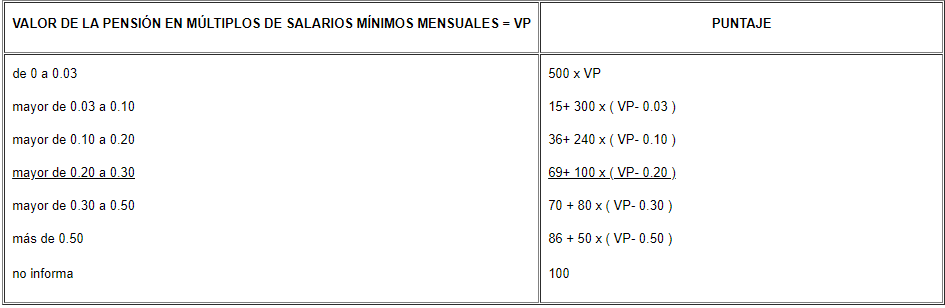
\includegraphics[width=1\linewidth]{ProtectoR/pension}

\}

\textbackslash{}caption\{Pensión. Recuperado de \url{http://www.legal.unal.edu.co/rlunal/home/doc.jsp?d_i=34298}\}\label{fig:unnamed-chunk-14}
\textbackslash{}end\{figure\}

de donde \(A_1=500\times 0,03=15\). Para el indicador estrato \(A_2\) la tabla \ref{tab:estrato} nos indica que \(A_2=30\). Siguiendo con el indicador \(A_3\) se asigna mediante la expresión
\[ A_3=9\times ING=9\times 3,33=55\]
donde \(ING\) son los ingresos mensuales expresados como un múltiplo del salario mínimo legal mensual vigente en el año respectivo.

\begin{figure}
 
 {\centering 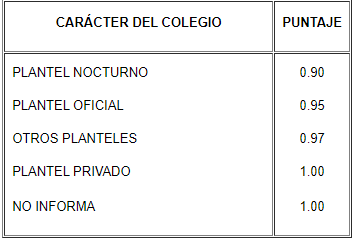
\includegraphics[width=0.5\linewidth]{ProtectoR/b1} 
 
 }
 
 \caption{$B_1$ Carácter del colegio.}\label{fig:unnamed-chunk-15}
 \end{figure}
 \begin{figure}
 
 {\centering 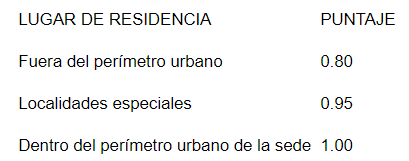
\includegraphics[width=0.5\linewidth]{ProtectoR/b2n} 
 
 }
 
 \caption{$B_2$ Lugar de residencia. }\label{fig:unnamed-chunk-16}
 \end{figure}
\begin{figure}

{\centering 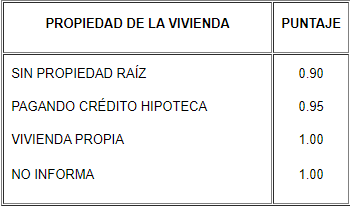
\includegraphics[width=0.5\linewidth]{ProtectoR/b3} 

}

\caption{$B_3$ Propiedad de la vivienda familiar.}\label{fig:unnamed-chunk-17}
\end{figure}

\begin{figure}

{\centering 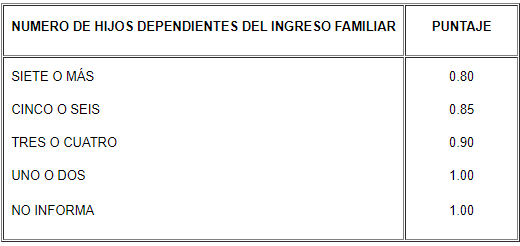
\includegraphics[width=0.5\linewidth]{ProtectoR/b4} 

}

\caption{$B_4$ Número de hijos dependientes del ingreso del hogar.}\label{fig:unnamed-chunk-18}
\end{figure}

Imágenes tomadas de \citet{BibEntry2021Maria}.

Como lo indica las tablas, se obtiene los puntajes \(B_1=0,95\), \(B_2=0,80\), \(B_3=1\) y \(B_4=1\) respectivamente. Utilizando la fórmula

\[\begin{eqnarray}
PBM&=&(0,4A_1+0,3A_2+0,3A_3)\times B_1 \times B_2 \times B_3 \times B_4\\
&=& (0,4(15)+0,3(30)+0,3(55))\times 0,95 \times 0,80 \times 1 \times 1\\
&=& 24
\end{eqnarray}\]

se llega a que la aspirante obtiene un puntaje de 24.

  \bibliography{biblio.bib,packages.bib}

\end{document}
